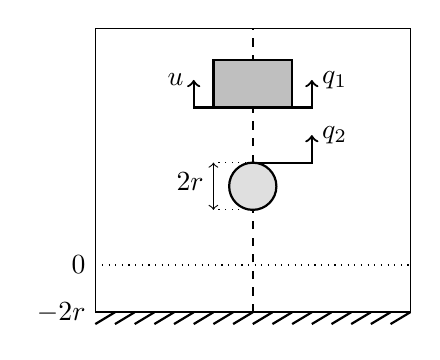
\begin{tikzpicture}
	%
	% axes
	\draw[thick] (0,-0.6)--(4,-0.6);
	\draw[dotted] (0,0) node[anchor = east] {\color{black}$0$}--(4,0);
	\draw[thick,dashed] (2,-0.6) -- (2,3);
	\draw (0,-0.6) node[anchor = east] {$-2r$} -- (4,-0.6) -- (4,3) -- (0,3) -- (0,-0.6);
	
	% robot
	\fill[gray!50, draw = black,thick] (1.5,2) rectangle (2.5,2.6);
	% ball
	\fill[gray!25, draw=black,thick] (2,1) circle (0.3);
	%	
	\draw[thick,->] (2.5,2) -- (2.75,2) -- (2.75,2.35) node[anchor=west] {$q_1$};
	\draw[thick,->] (1.5,2) -- (1.25,2) -- (1.25,2.35) node[anchor=east] {$u$};
	\draw[thick,->] (2,1.3) -- (2.75,1.3) -- (2.75,1.65) node[anchor=west] {$q_2$};
	%
	\draw[dotted] (2,1.3) -- (1.5,1.3);
	\draw[dotted] (2,0.7) -- (1.5,0.7);
	\draw[<->] (1.5,0.7) -- (1.5,1.3)  node[anchor=north east] {$2r$};
	%
	\foreach \x in {0,0.25,0.5,0.75,1,1.25,1.5,1.75,2,2.25,2.5,2.75,3,3.25,3.5,3.75}
	\draw[thick] (\x,-0.75) -- (\x+0.25,-0.6);
\end{tikzpicture}